
{
    The YOLOv8 training curves, are a visual representation that serves as a snapshot of the model development.
}

\begin{figure}[!p]
	\centering
	\begin{subfigure}[b]{\textwidth}
		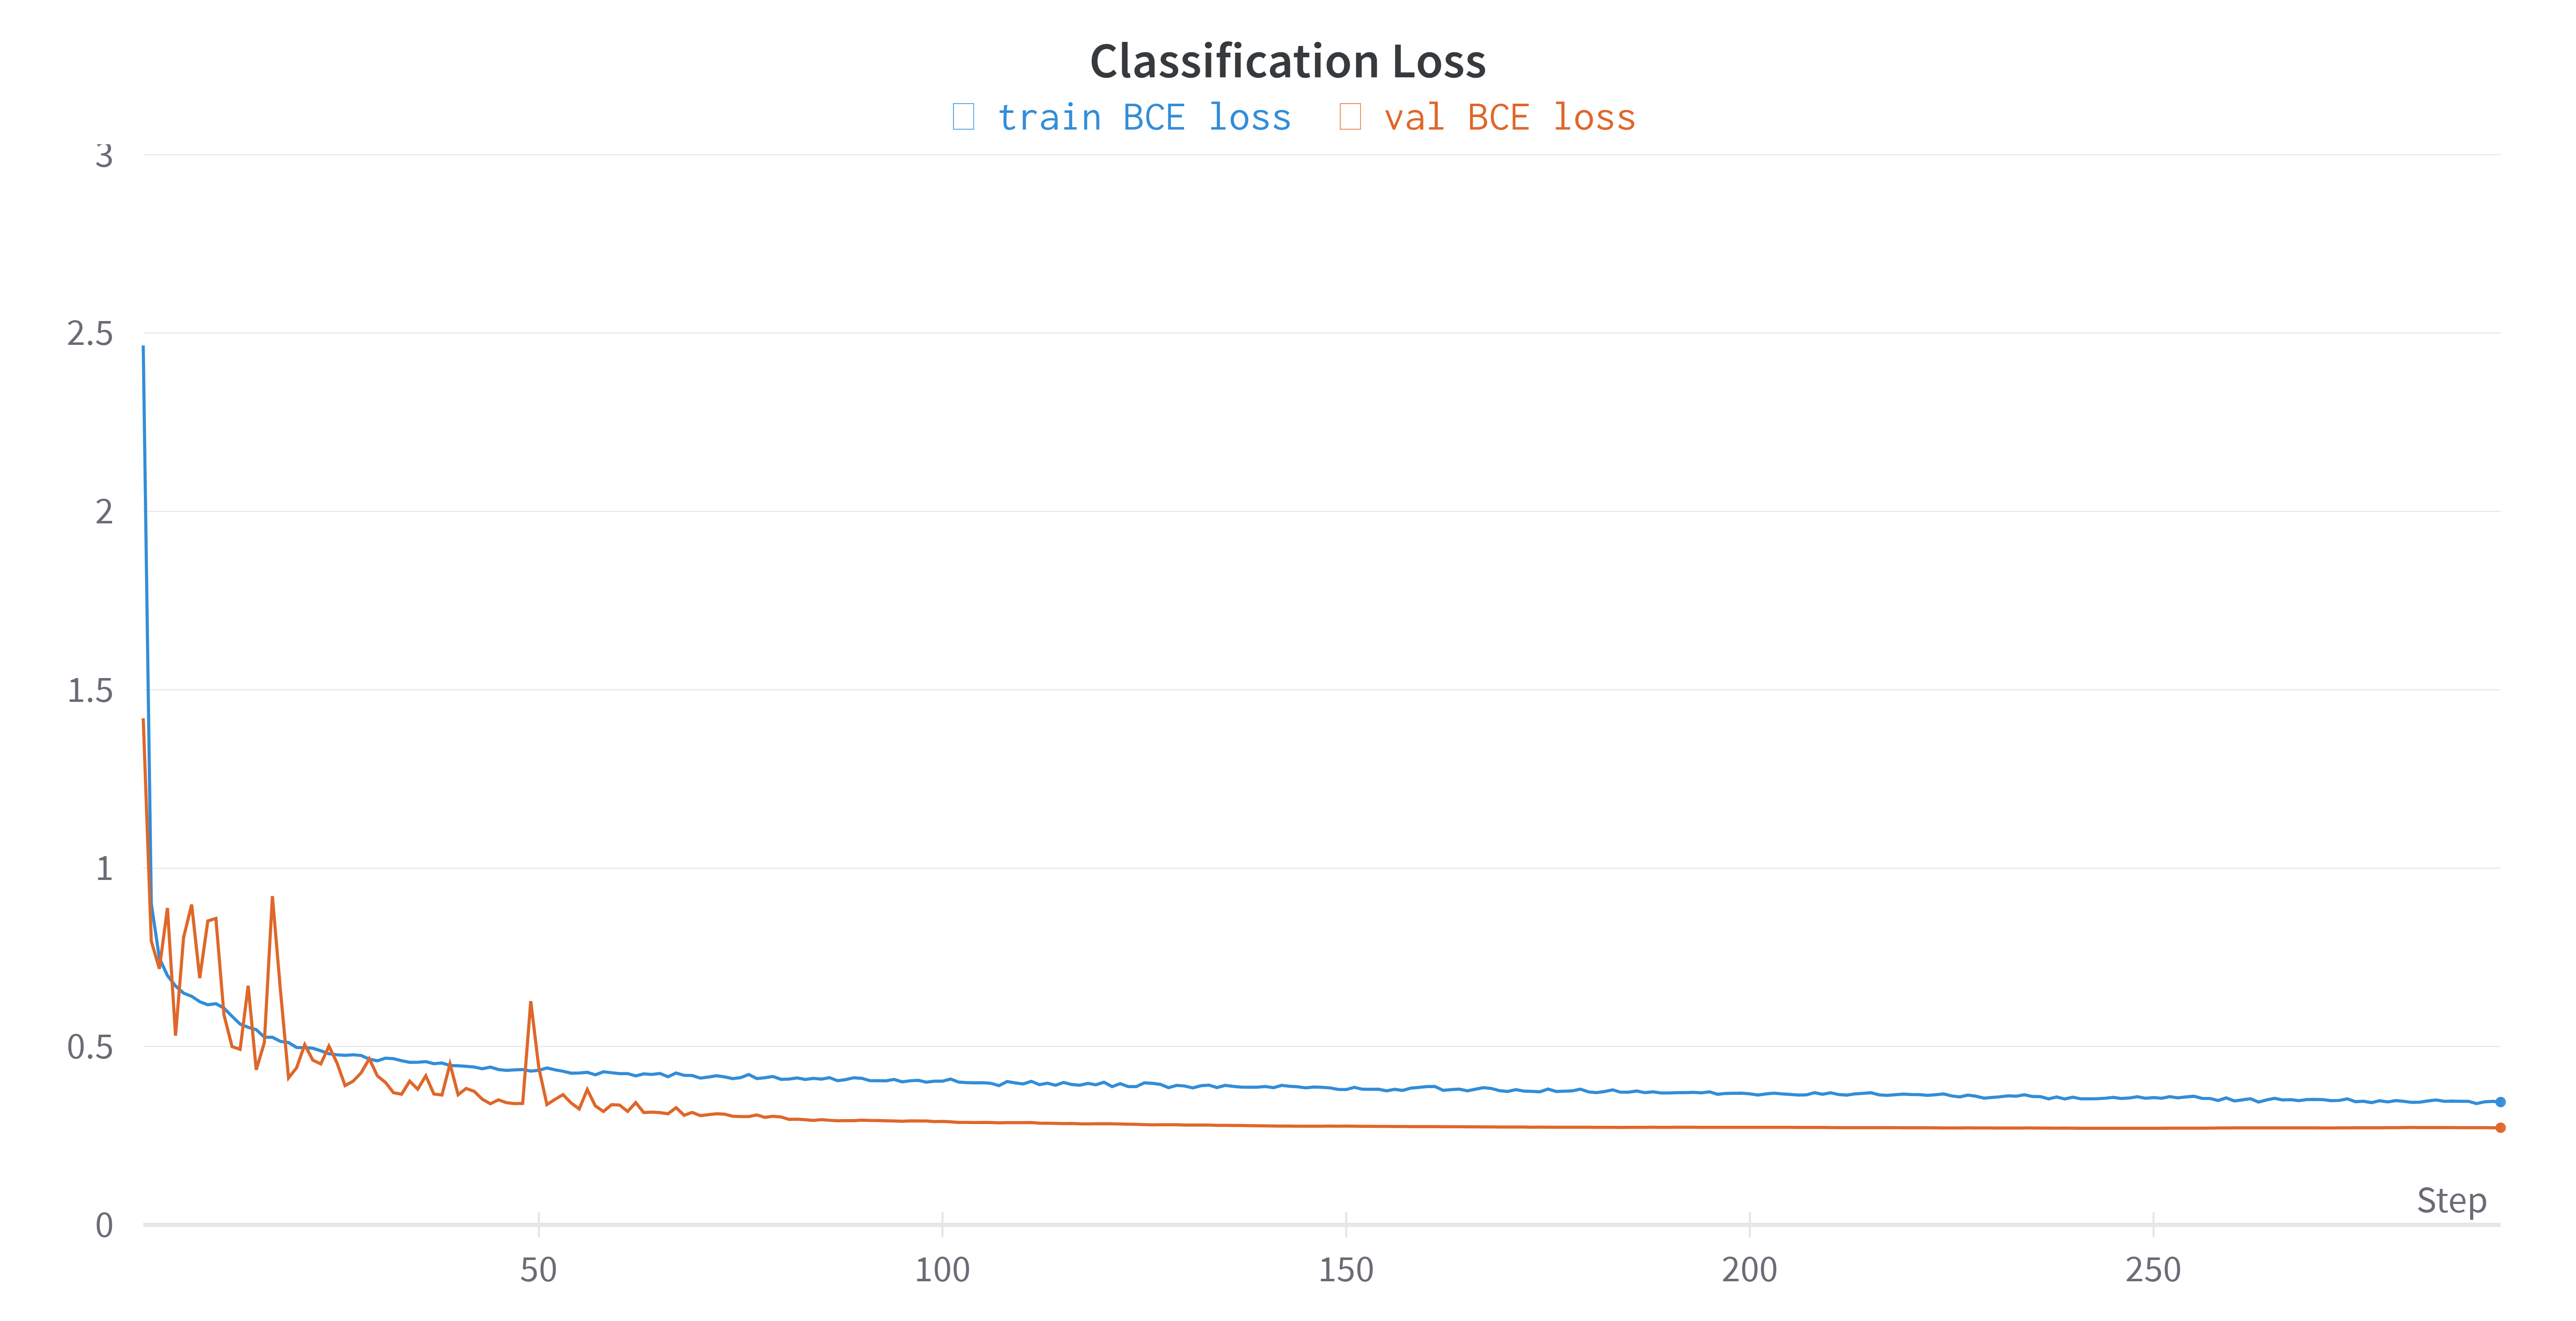
\includegraphics[width=\textwidth]{figures/06_results/ClassLossDetector.png}
		\caption{\footnotesize{Train and validation curves for the class classification loss.}}
		\label{fig:detector_class_loss}
	\end{subfigure}
	\begin{subfigure}[b]{\textwidth}
		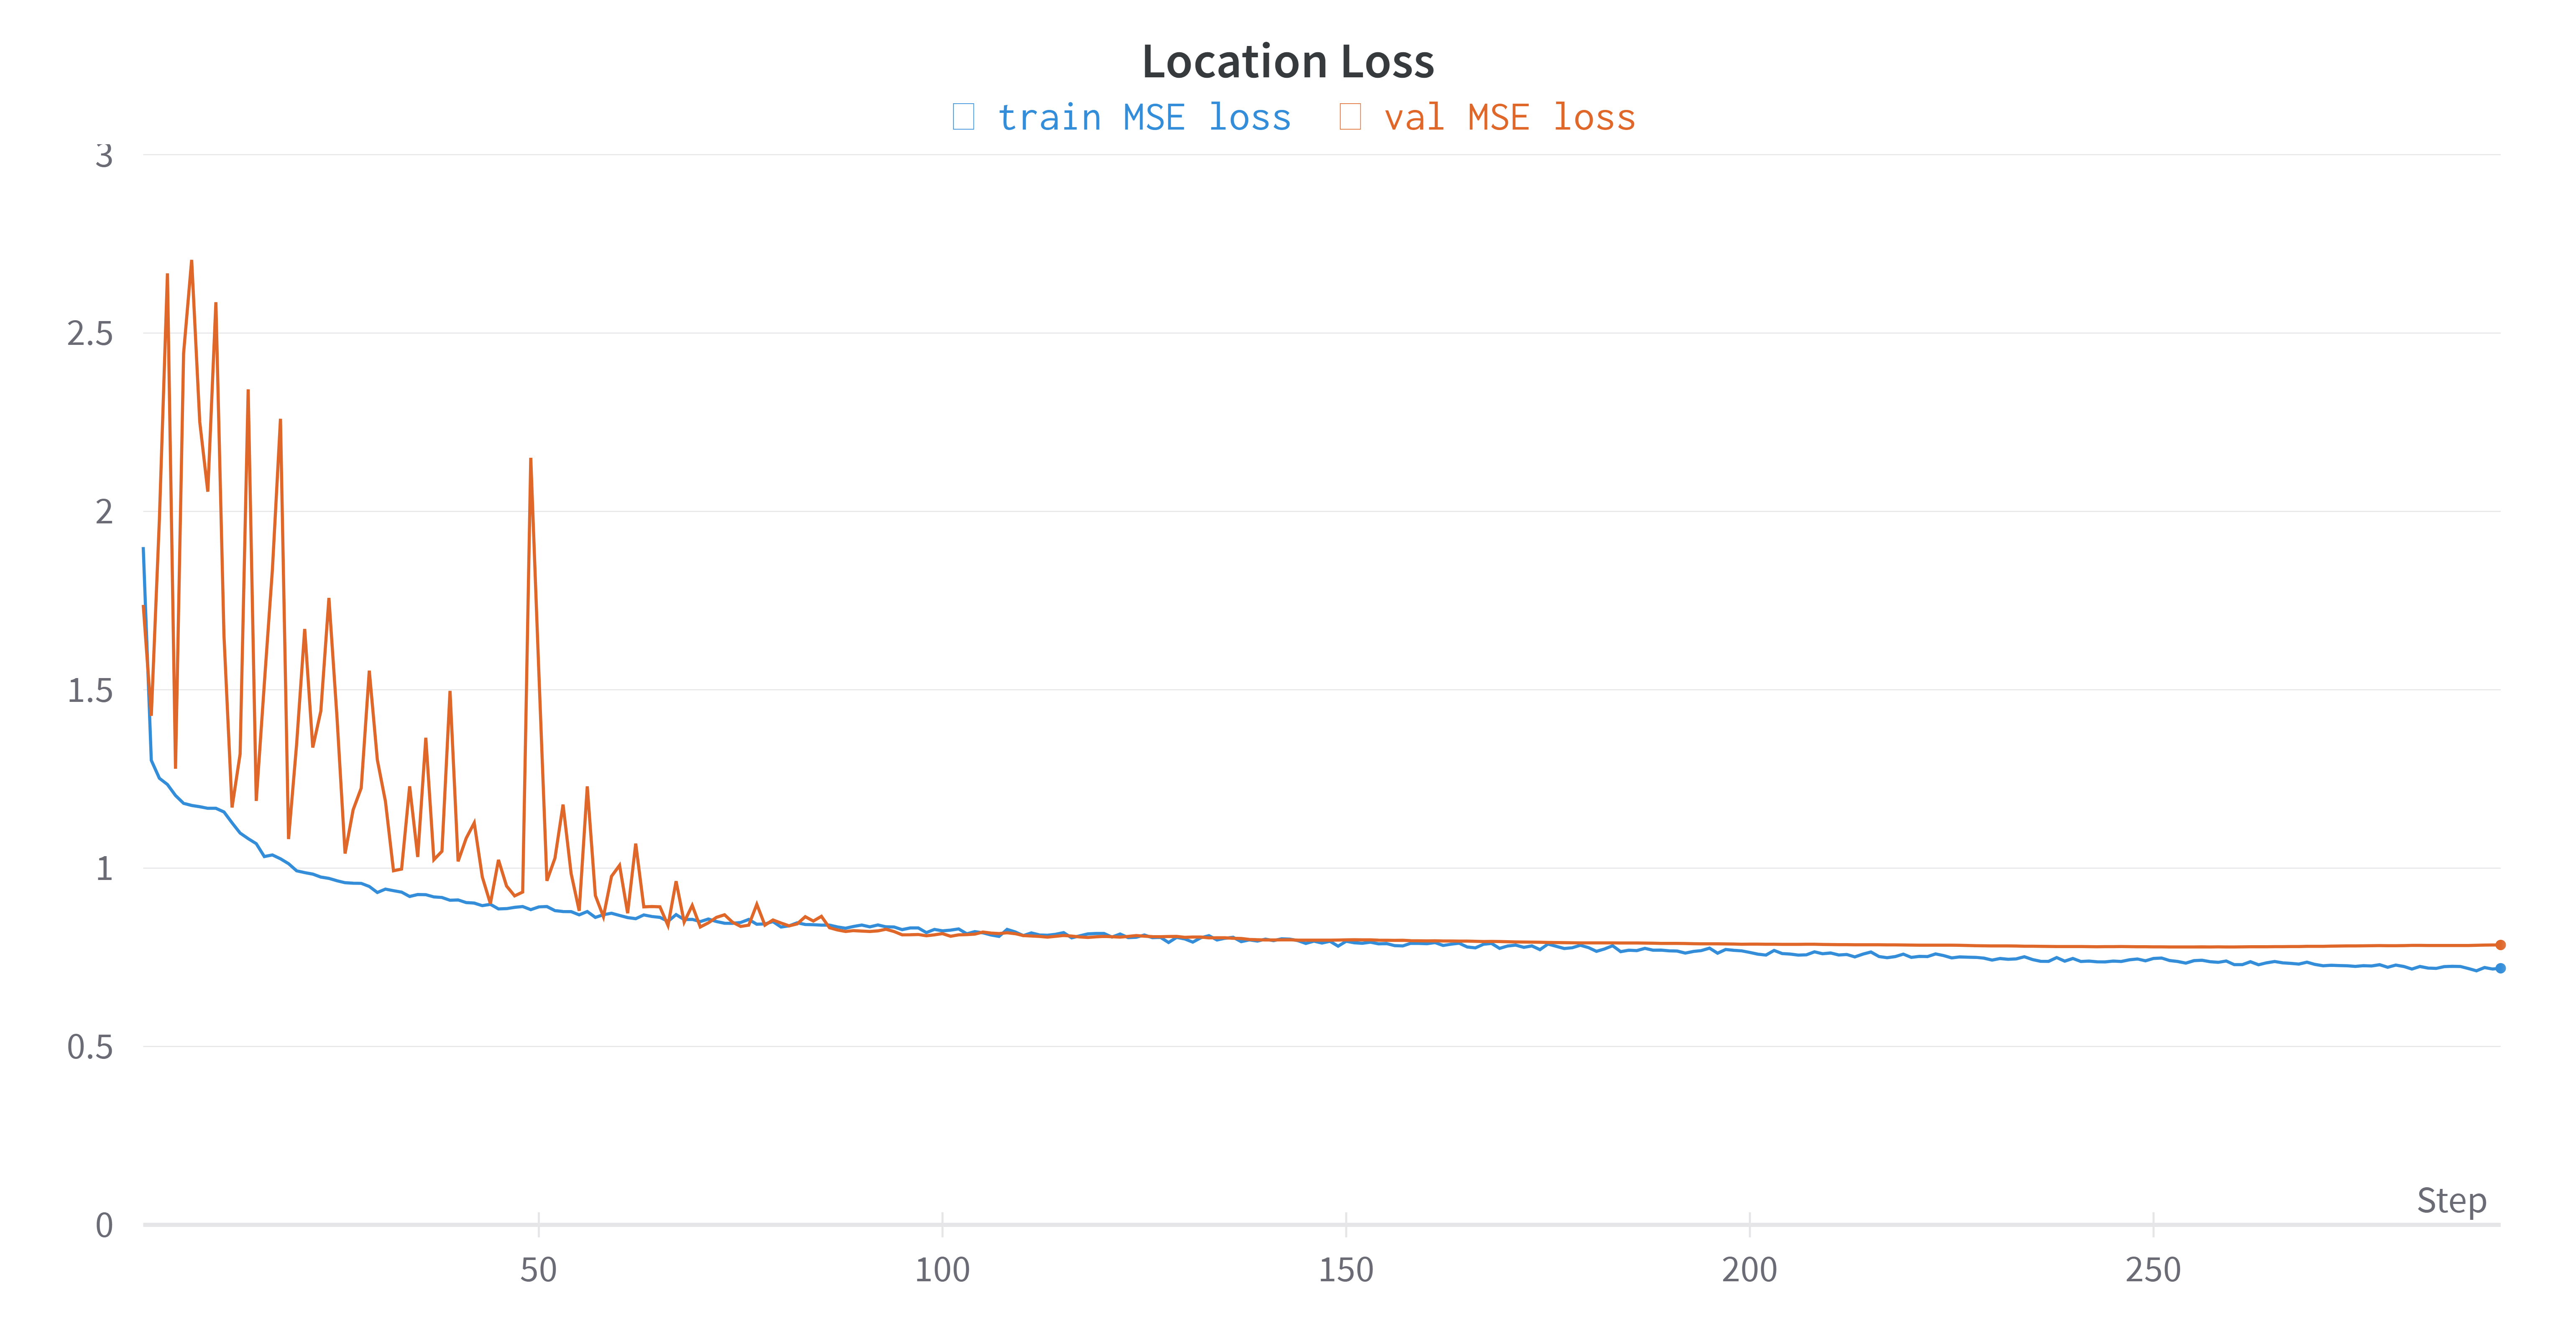
\includegraphics[width=\textwidth]{figures/06_results/LocationLossDetector.png}
		\caption{\footnotesize{Train and validation curves for the object location loss.}}
		\label{fig:detector_location_loss}
	\end{subfigure}
	
	\caption[Train and validation loss curves of YOLOv8]{\footnotesize{Train and validation loss curves of YOLOv8.}}
	\label{fig:yolov8 train curves}
\end{figure}

{
    From the curves on Figure \ref{fig:yolov8 train curves}, it can be seen the learning process starts fluctuating only on validation because the model is not optimized and the validation contains some randomness. 
	As the training advances, the validation curve stabilizes and slowly improves until the epoch 243; at the epoch 293 (of a maximum of 500) the trainer program early stopped the training. 
    The training ended successfully without overfitting.
}

%\begin{figure}[!p]
%    \centering
%    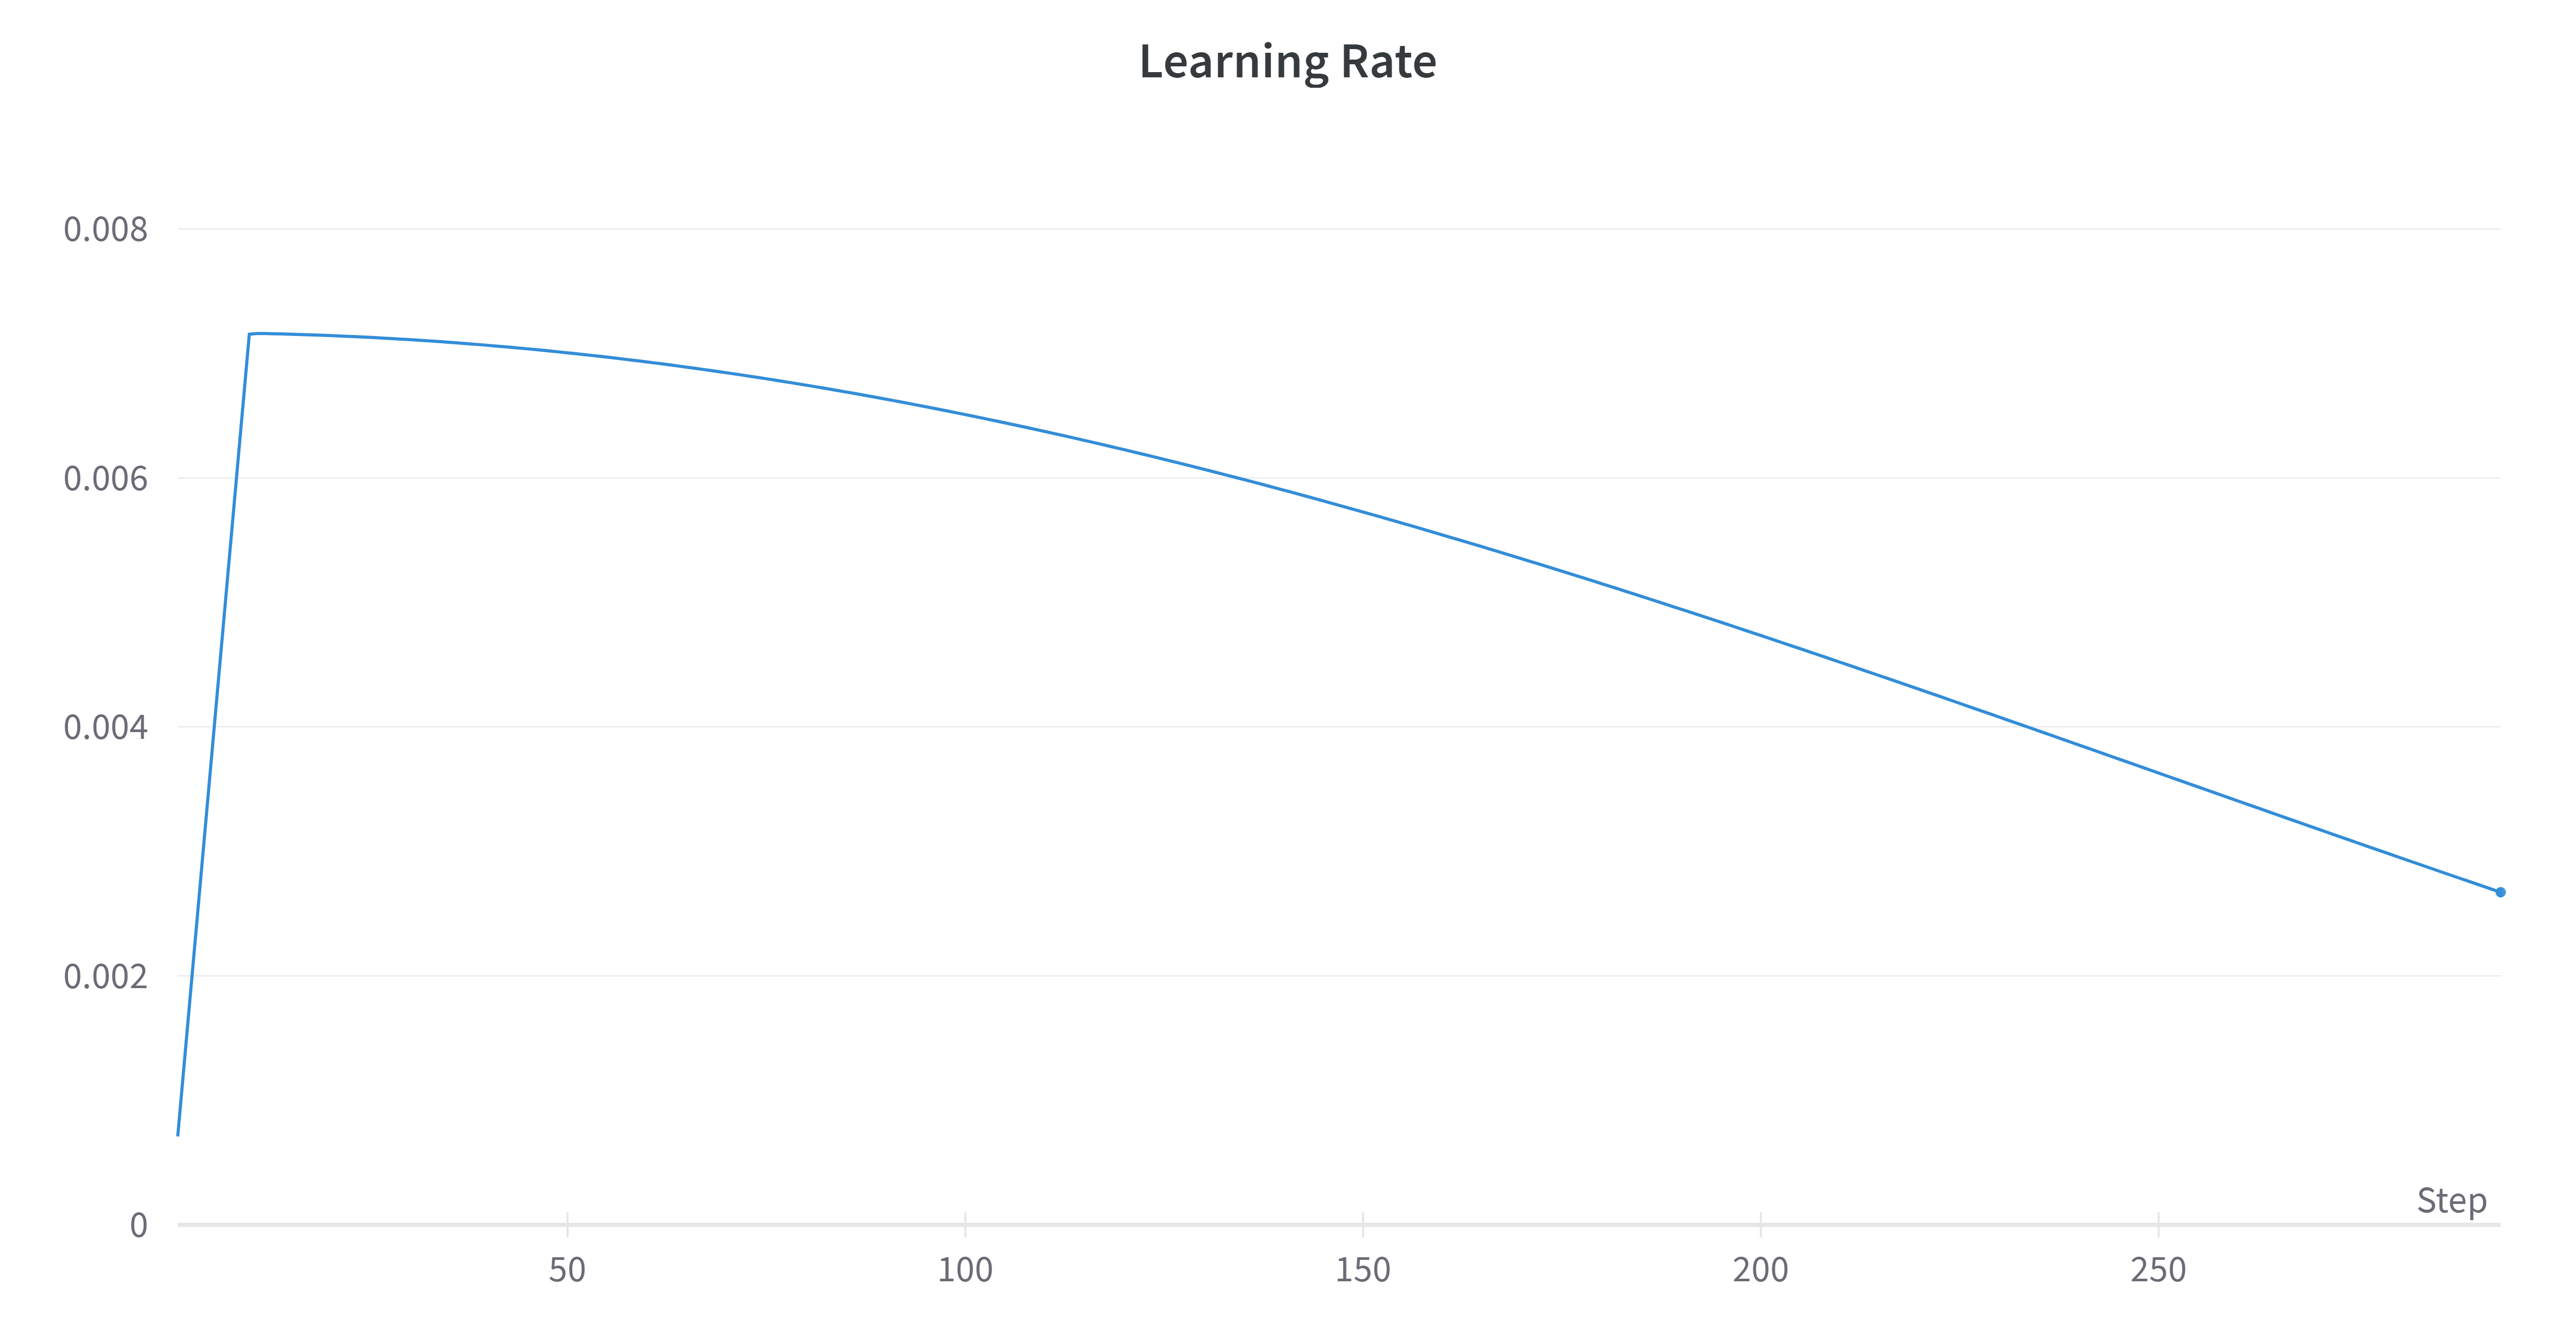
\includegraphics[width=0.45\textwidth]{figures/06_results/LearningRateDetector.png}
%    \caption[Learning rate curve of YOLOv8]{\footnotesize{Learning rate curve for the YOLOv8 training.}}
%    \label{fig:detector_learning_rate}
%\end{figure}

{
    Additionally, it was seen that, when adding more difficult data, the model reached a better solution\footnote{This result is valid because the ampliation of the validation dataset increased the difficulty (from a dataset of only one ant to a dataset with multiple ants interacting in groups), however, it would be better to repeat the curves with a unique version of the validation dataset.} on the increased dataset. 
    The validation \ac{mAP}@50-95 curves on Figure \ref{fig:validation mAP50-95} illustrates this statement, where both curves have similar shapes but different endpoints.
}

\begin{figure}[!p]
	\centering
	\begin{subfigure}[]{0.45\textwidth}
		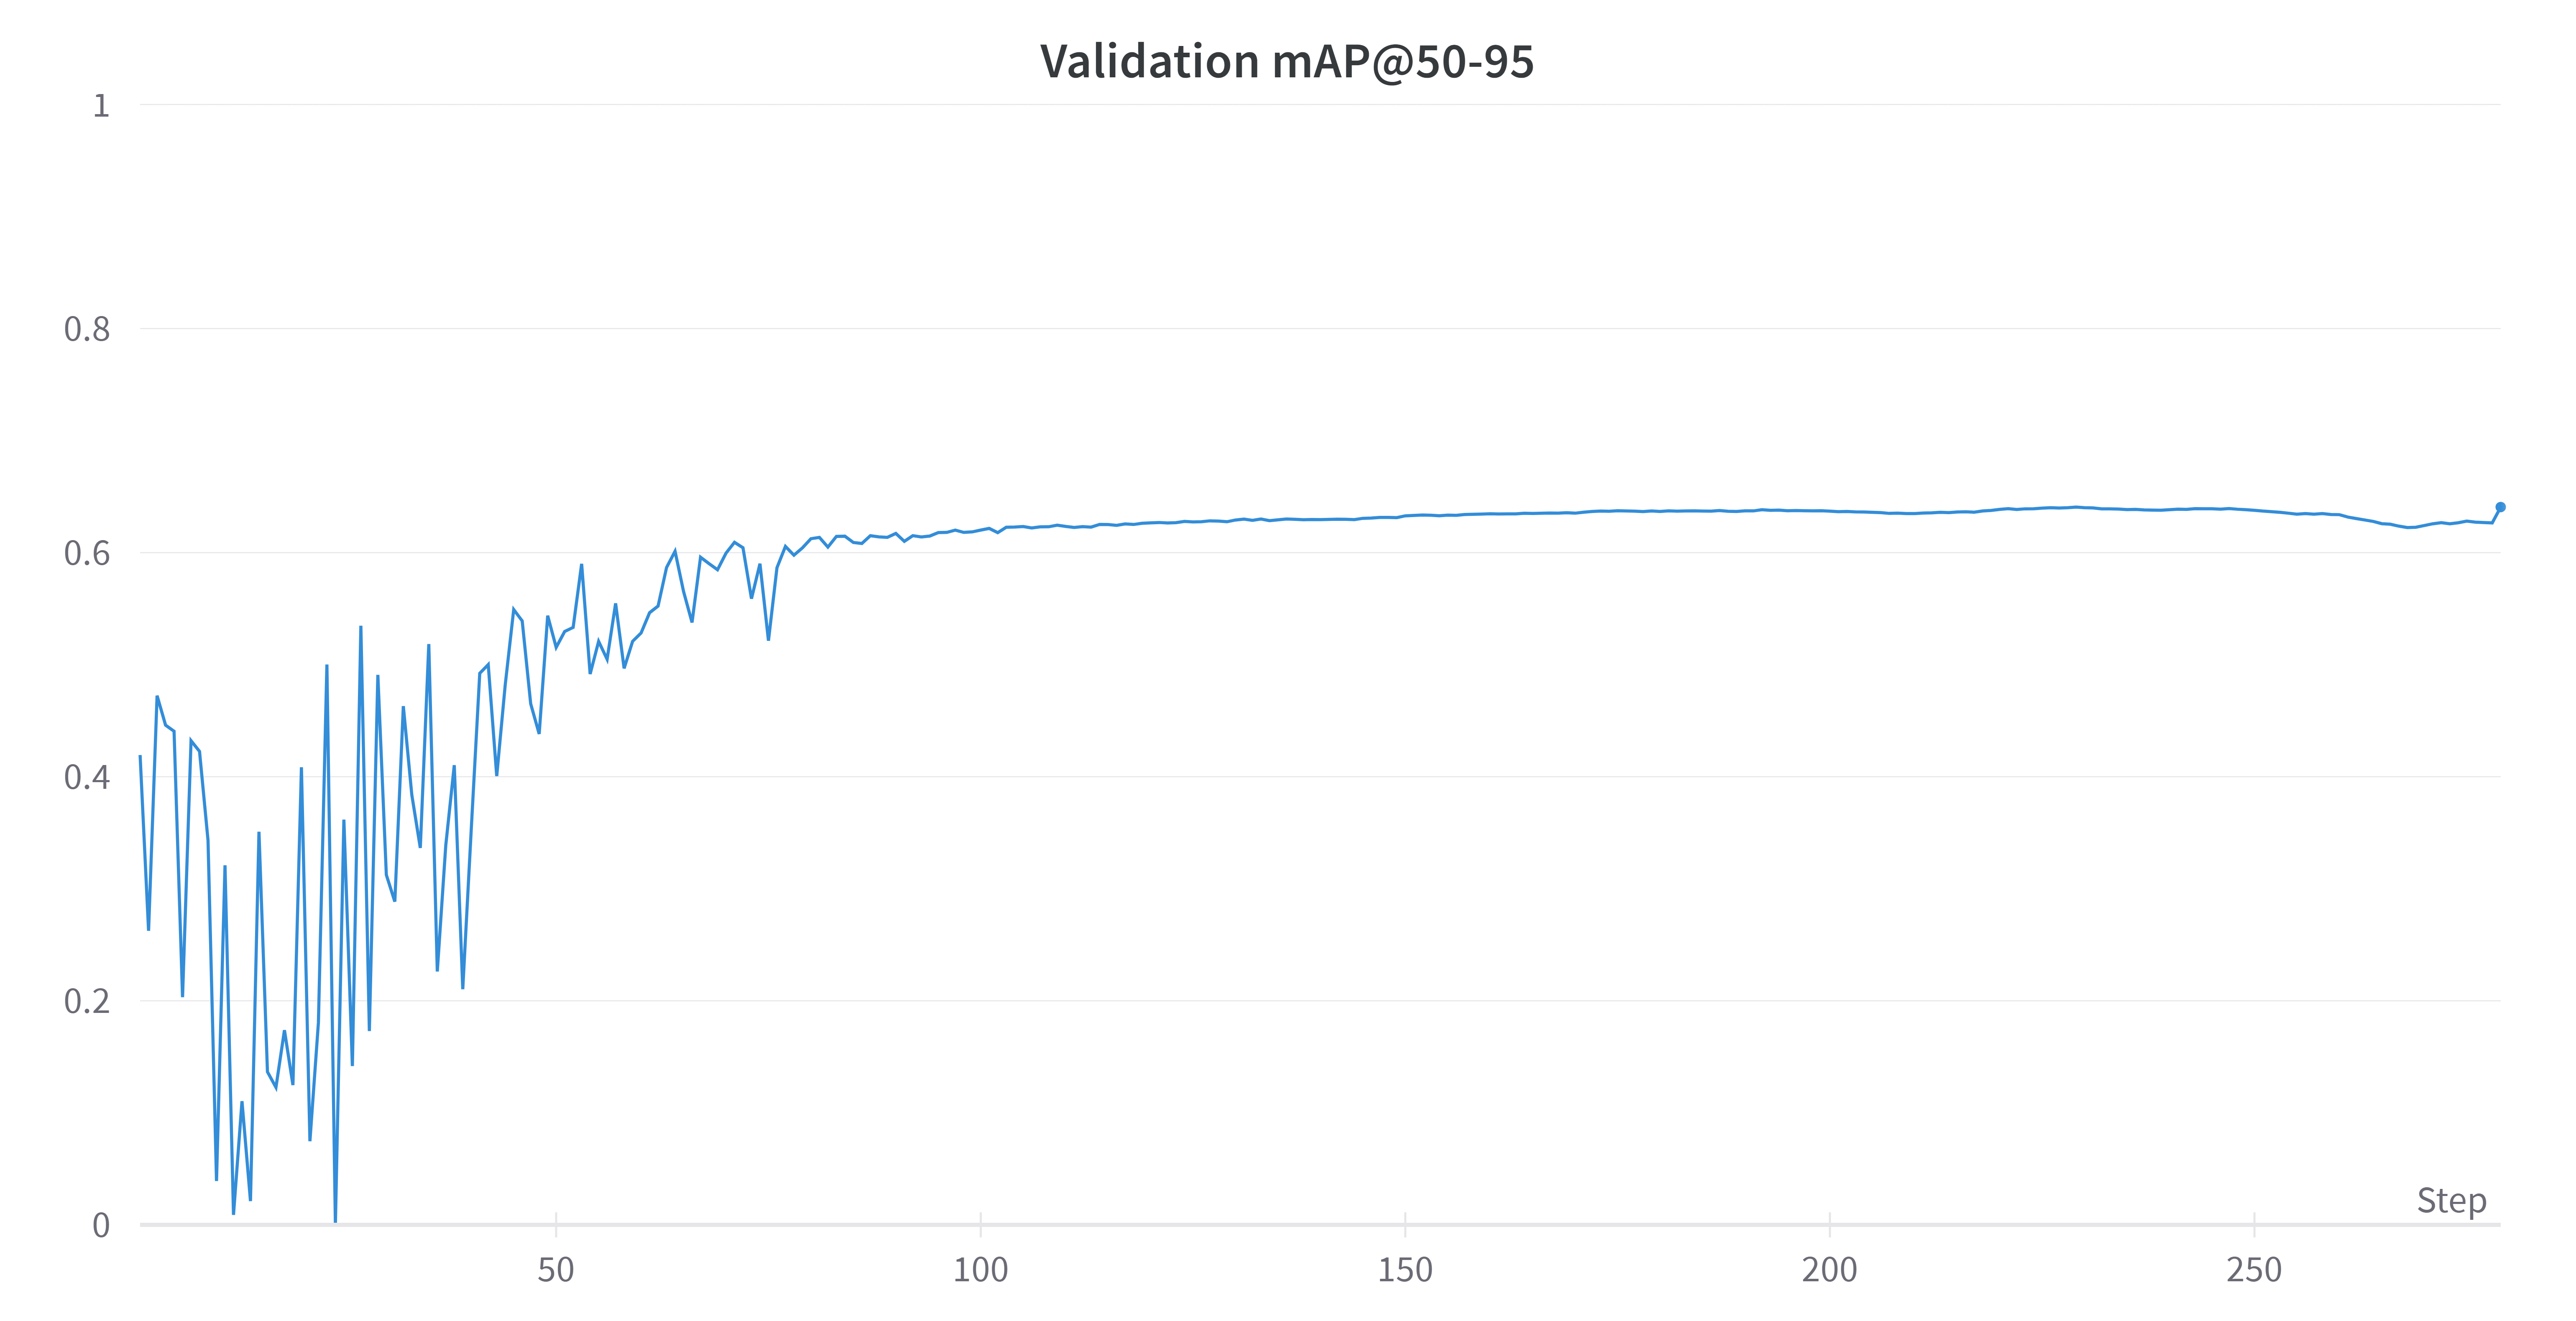
\includegraphics[width=\textwidth]{figures/06_results/mAP5095DetectorInitial.png}
		\caption{\footnotesize{Validation mAP@50-95 curves of YOLOv8 with the smaller dataset.}}
		\label{fig:validation mAP50-95 Initial}
	\end{subfigure}
	\begin{subfigure}[]{0.45\textwidth}
		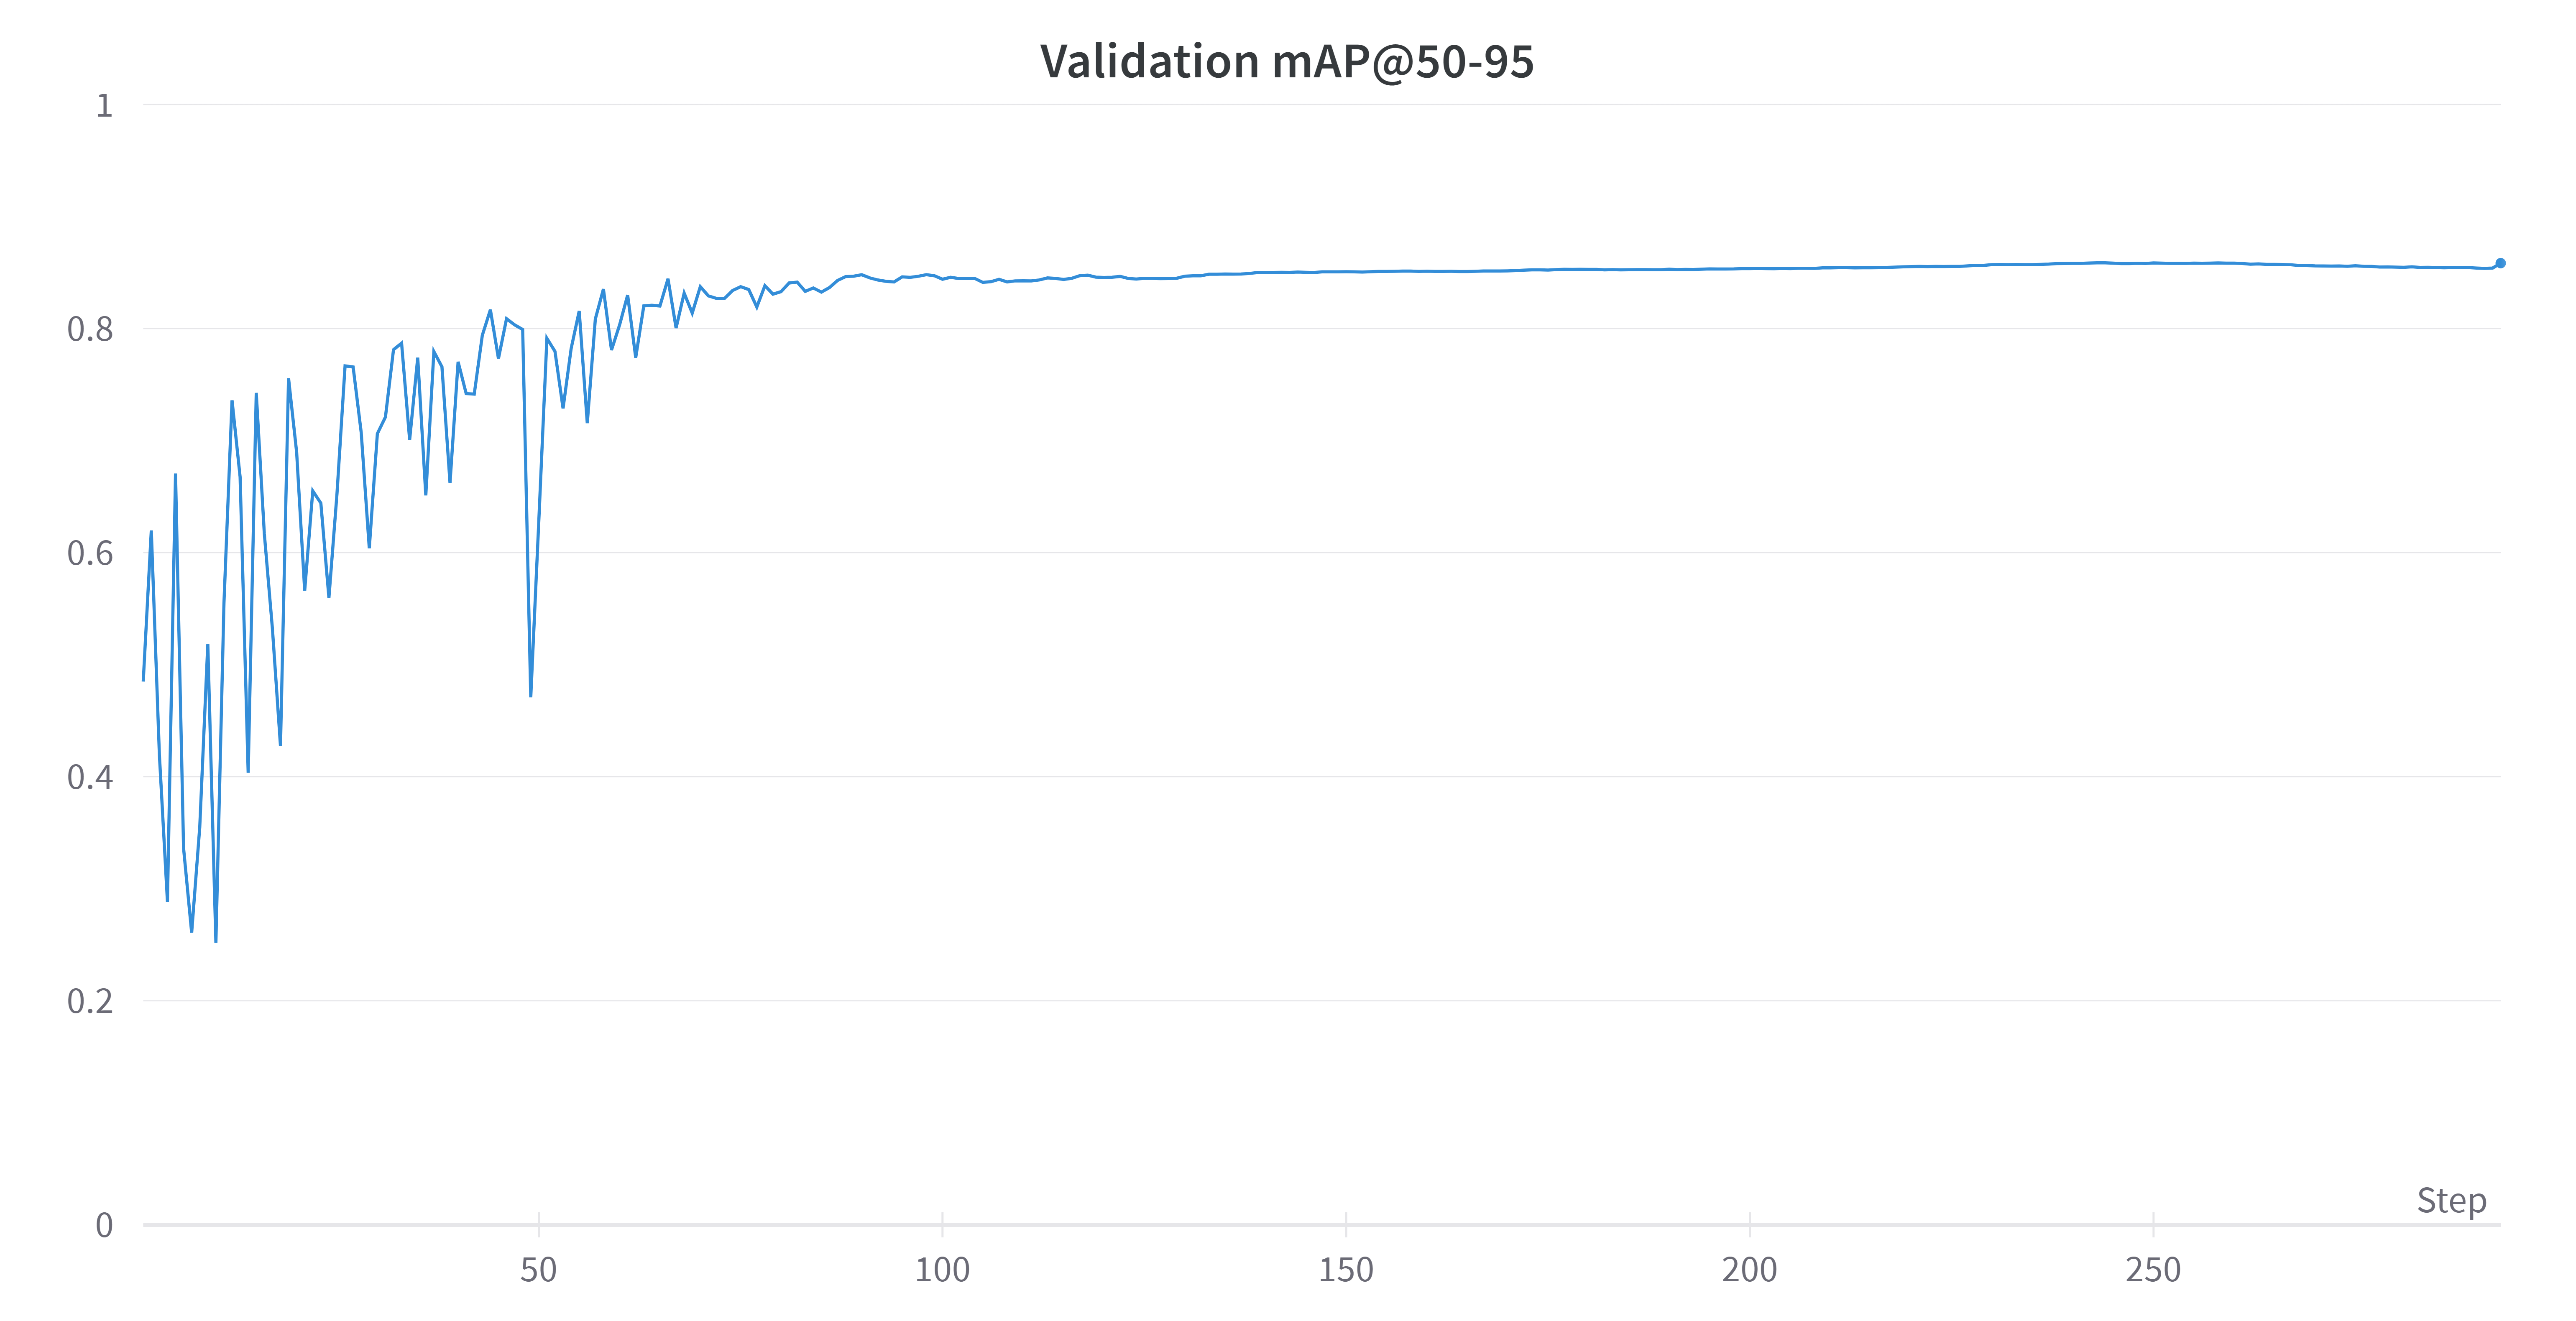
\includegraphics[width=\textwidth]{figures/06_results/mAP5095Detector.png}
		\caption{\footnotesize{Validation mAP@50-95 curves of YOLOv8 with the bigger and harder dataset.}}
		\label{fig:validation mAP50-95 Final}
	\end{subfigure}
	
	\caption[Validation mAP@50-95 curves of YOLOv8]{\footnotesize{Validation mAP@50-95 curves of YOLOv8 trained and validated with a dataset and a previous version of the same dataset.}}
	\label{fig:validation mAP50-95}
\end{figure}

{
    Figures \ref{fig:detector_precision}, \ref{fig:detector_recall} and \ref{fig:detector_f1score} present the precision, recall and F1-Score metrics, assessed at various confidence thresholds. 
    When transitioning from detection to tracking, the primary objective is to attain a high recall rate to minimize the loss of ants during the tracking phase. This approach is rooted in the rationale that spurious false positives can be subsequently filtered out by the tracking model.
}

{
	As seen on Figure \ref{fig:detector_f1score}, the optimal F1-Score on the validation set occurs at 0.5. 
    For the tracking model, the minimum detection confidence parameter was set to 0.4. 
    This choice deliberately shift towards a higher recall because the tracking process is able to filter spurious false positives out.
}

{
    Furthermore, the low-high confidence threshold was set at 0.8. 
    At this threshold, the impact of a reduced recall on the F1-Score becomes noticeable, prompting a thoughtful balance in model performance.
}

{
    The training of the \ac{YOLOv8n} model was performed on CALCULA, the computing server from the \ac{TSC} department of the \ac{UPC}, using 1 GPU NVIDIA GeForce RTX 3090 with 24 GB of memory available, 16 cores of CPU and 32 GB of RAM. With this setting and the previously explained hyperparameters (on Table \ref{tab:detection hyperparameters}), the longest training duration was smaller than 7 hours.
}

\begin{figure}[!p]
	\centering
	\begin{subfigure}[]{0.45\textwidth}
        \centering
		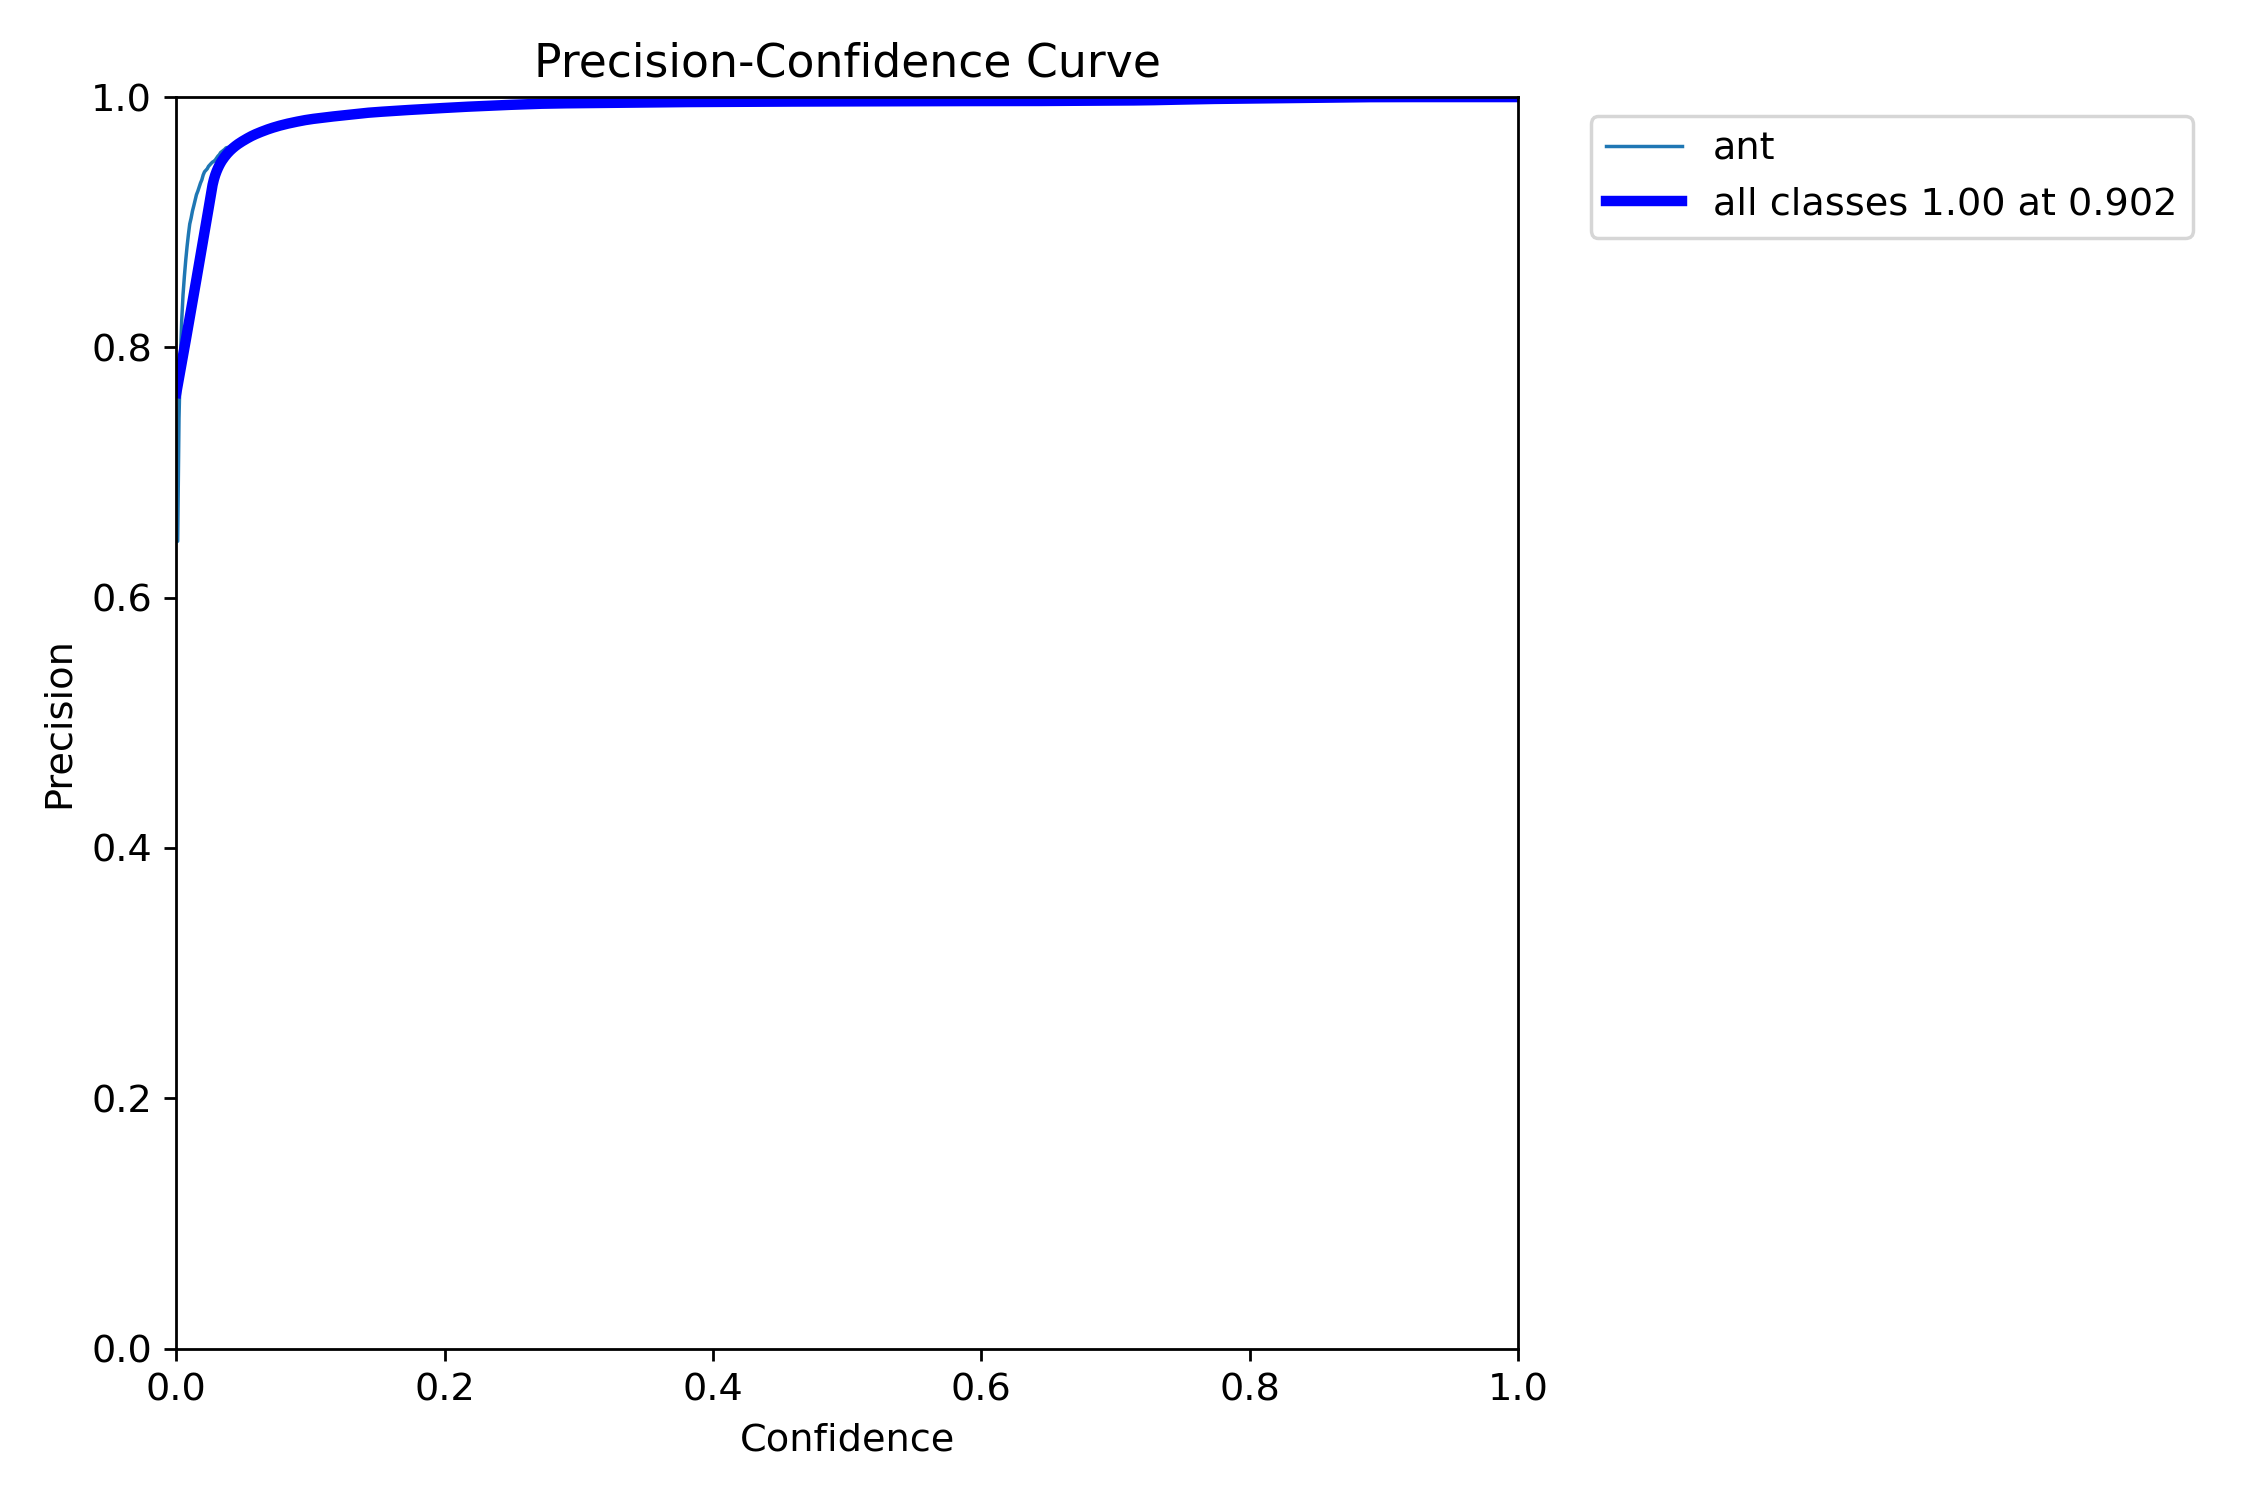
\includegraphics[width=\textwidth]{figures/06_results/PrecisionCurveDetector.png}
        \caption[Precision-Confidence curve of YOLOv8]{\footnotesize{Precision-Confidence curve.}}
        \label{fig:detector_precision}
	\end{subfigure}
	\begin{subfigure}[]{0.45\textwidth}
        \centering
		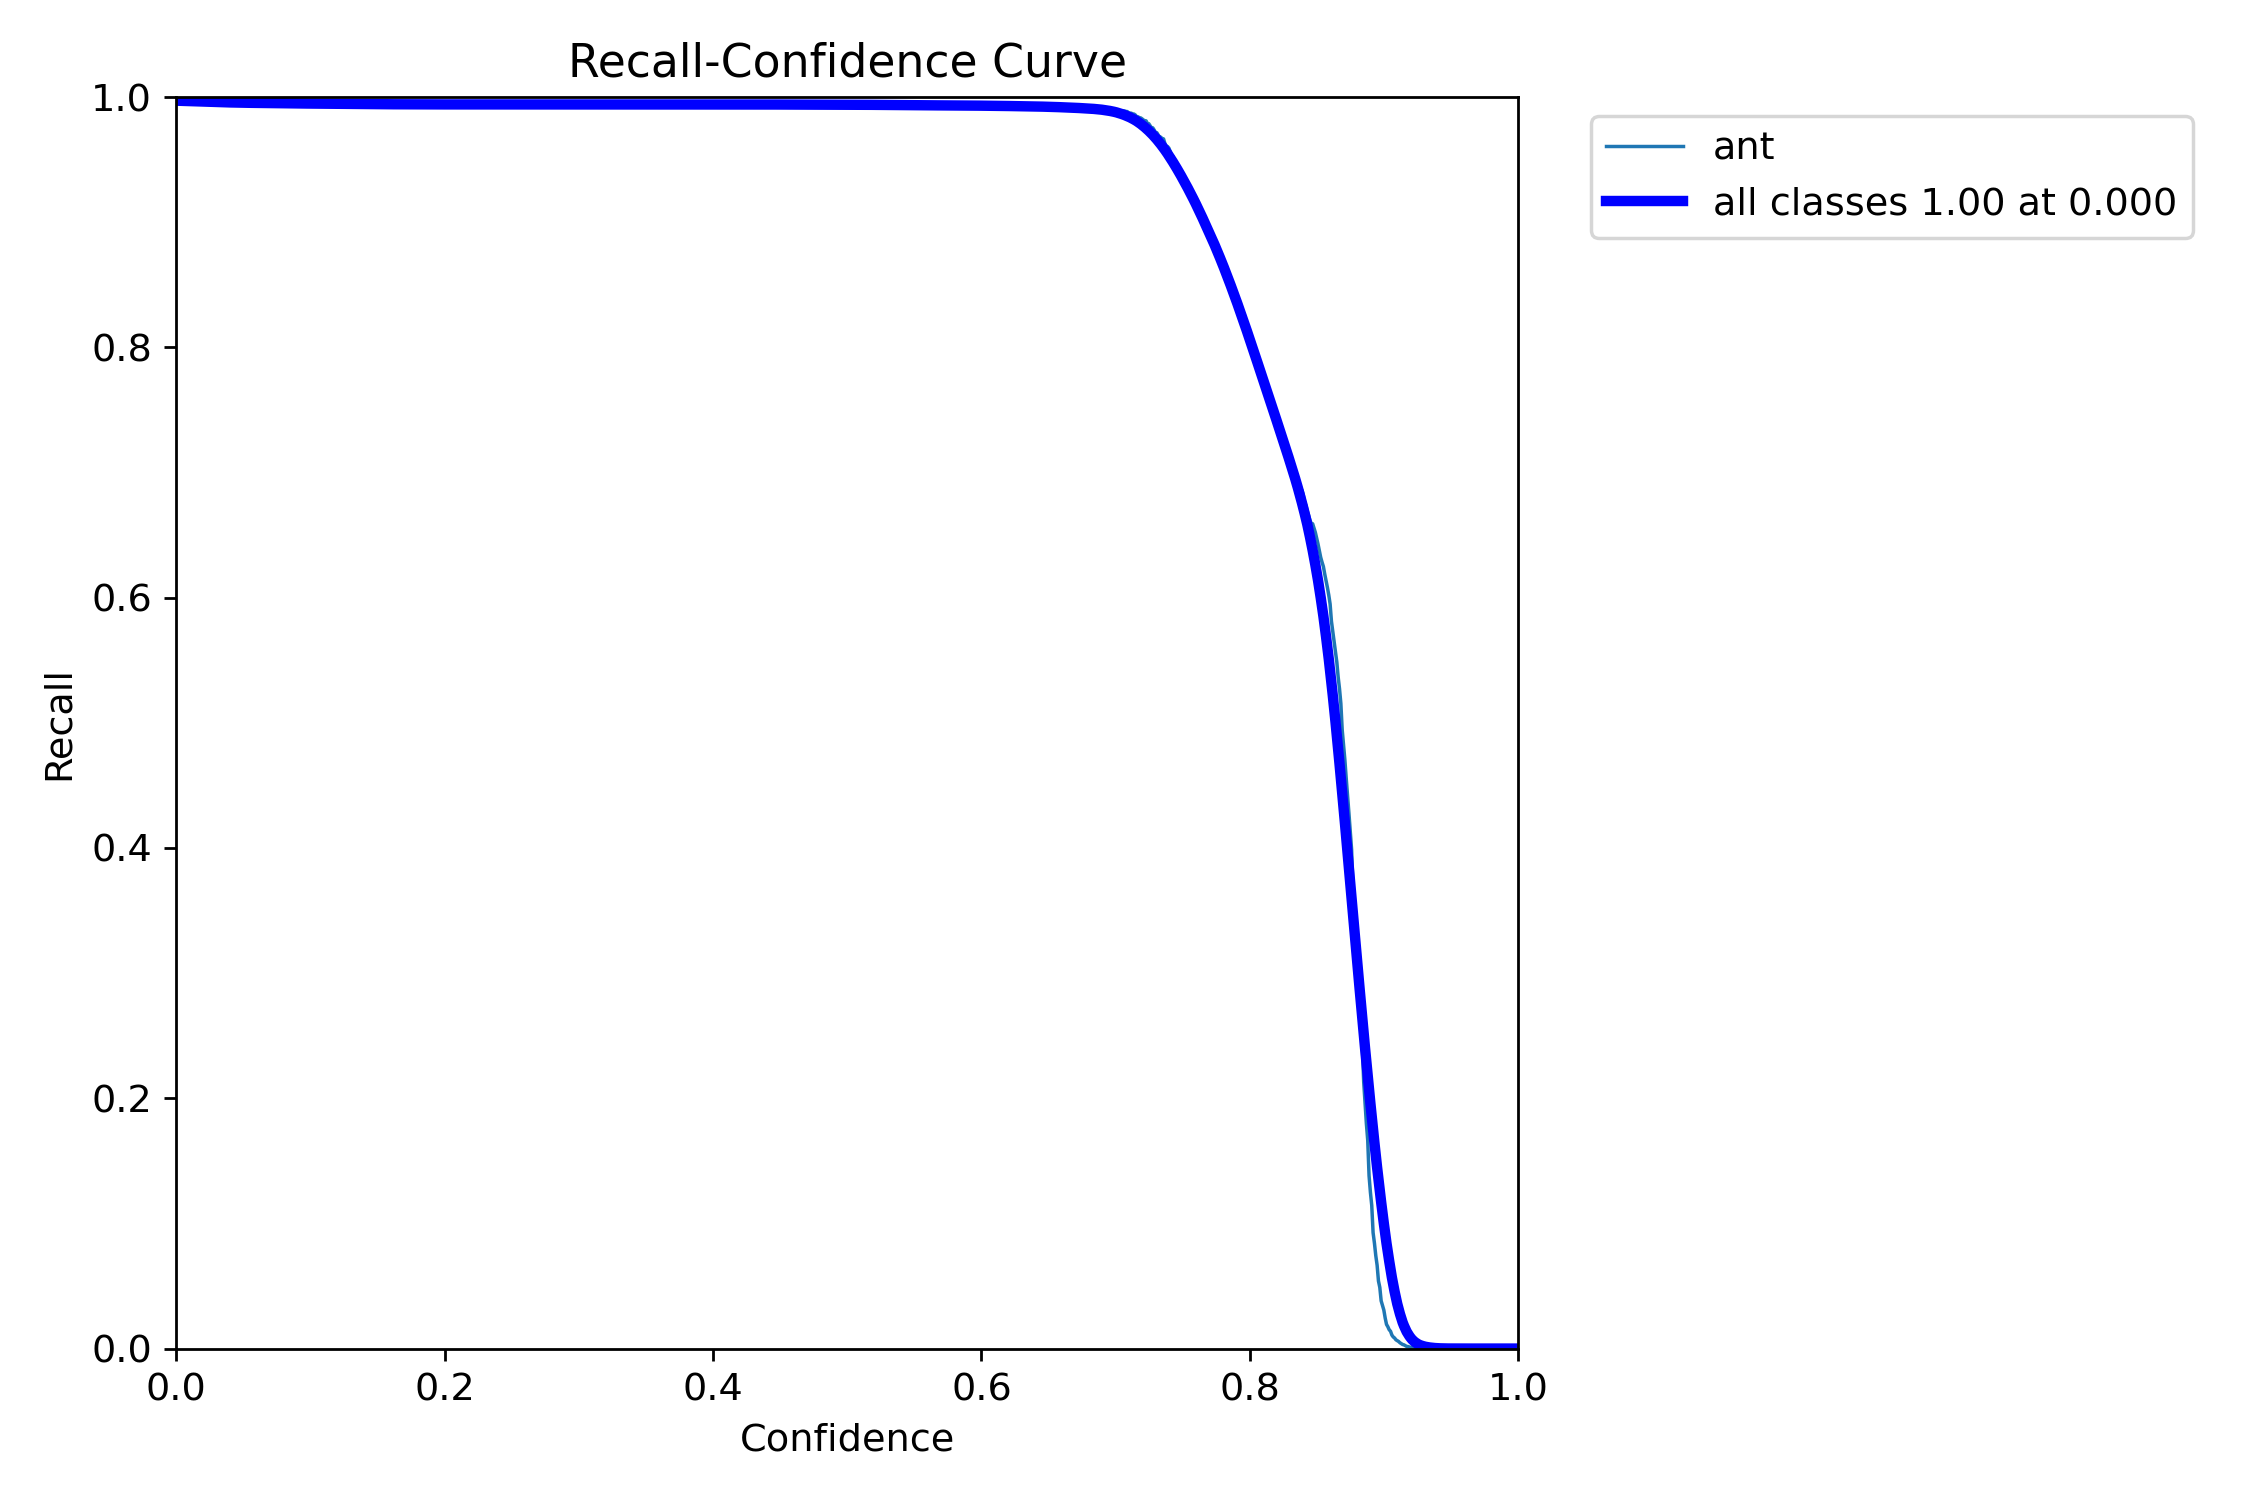
\includegraphics[width=\textwidth]{figures/06_results/RecallCurveDetector.png}
        \caption[Recall-Confidence curve of YOLOv8]{\footnotesize{Recall-Confidence curve.}}
        \label{fig:detector_recall}
	\end{subfigure}

    \begin{subfigure}[]{0.45\textwidth}
        \centering
		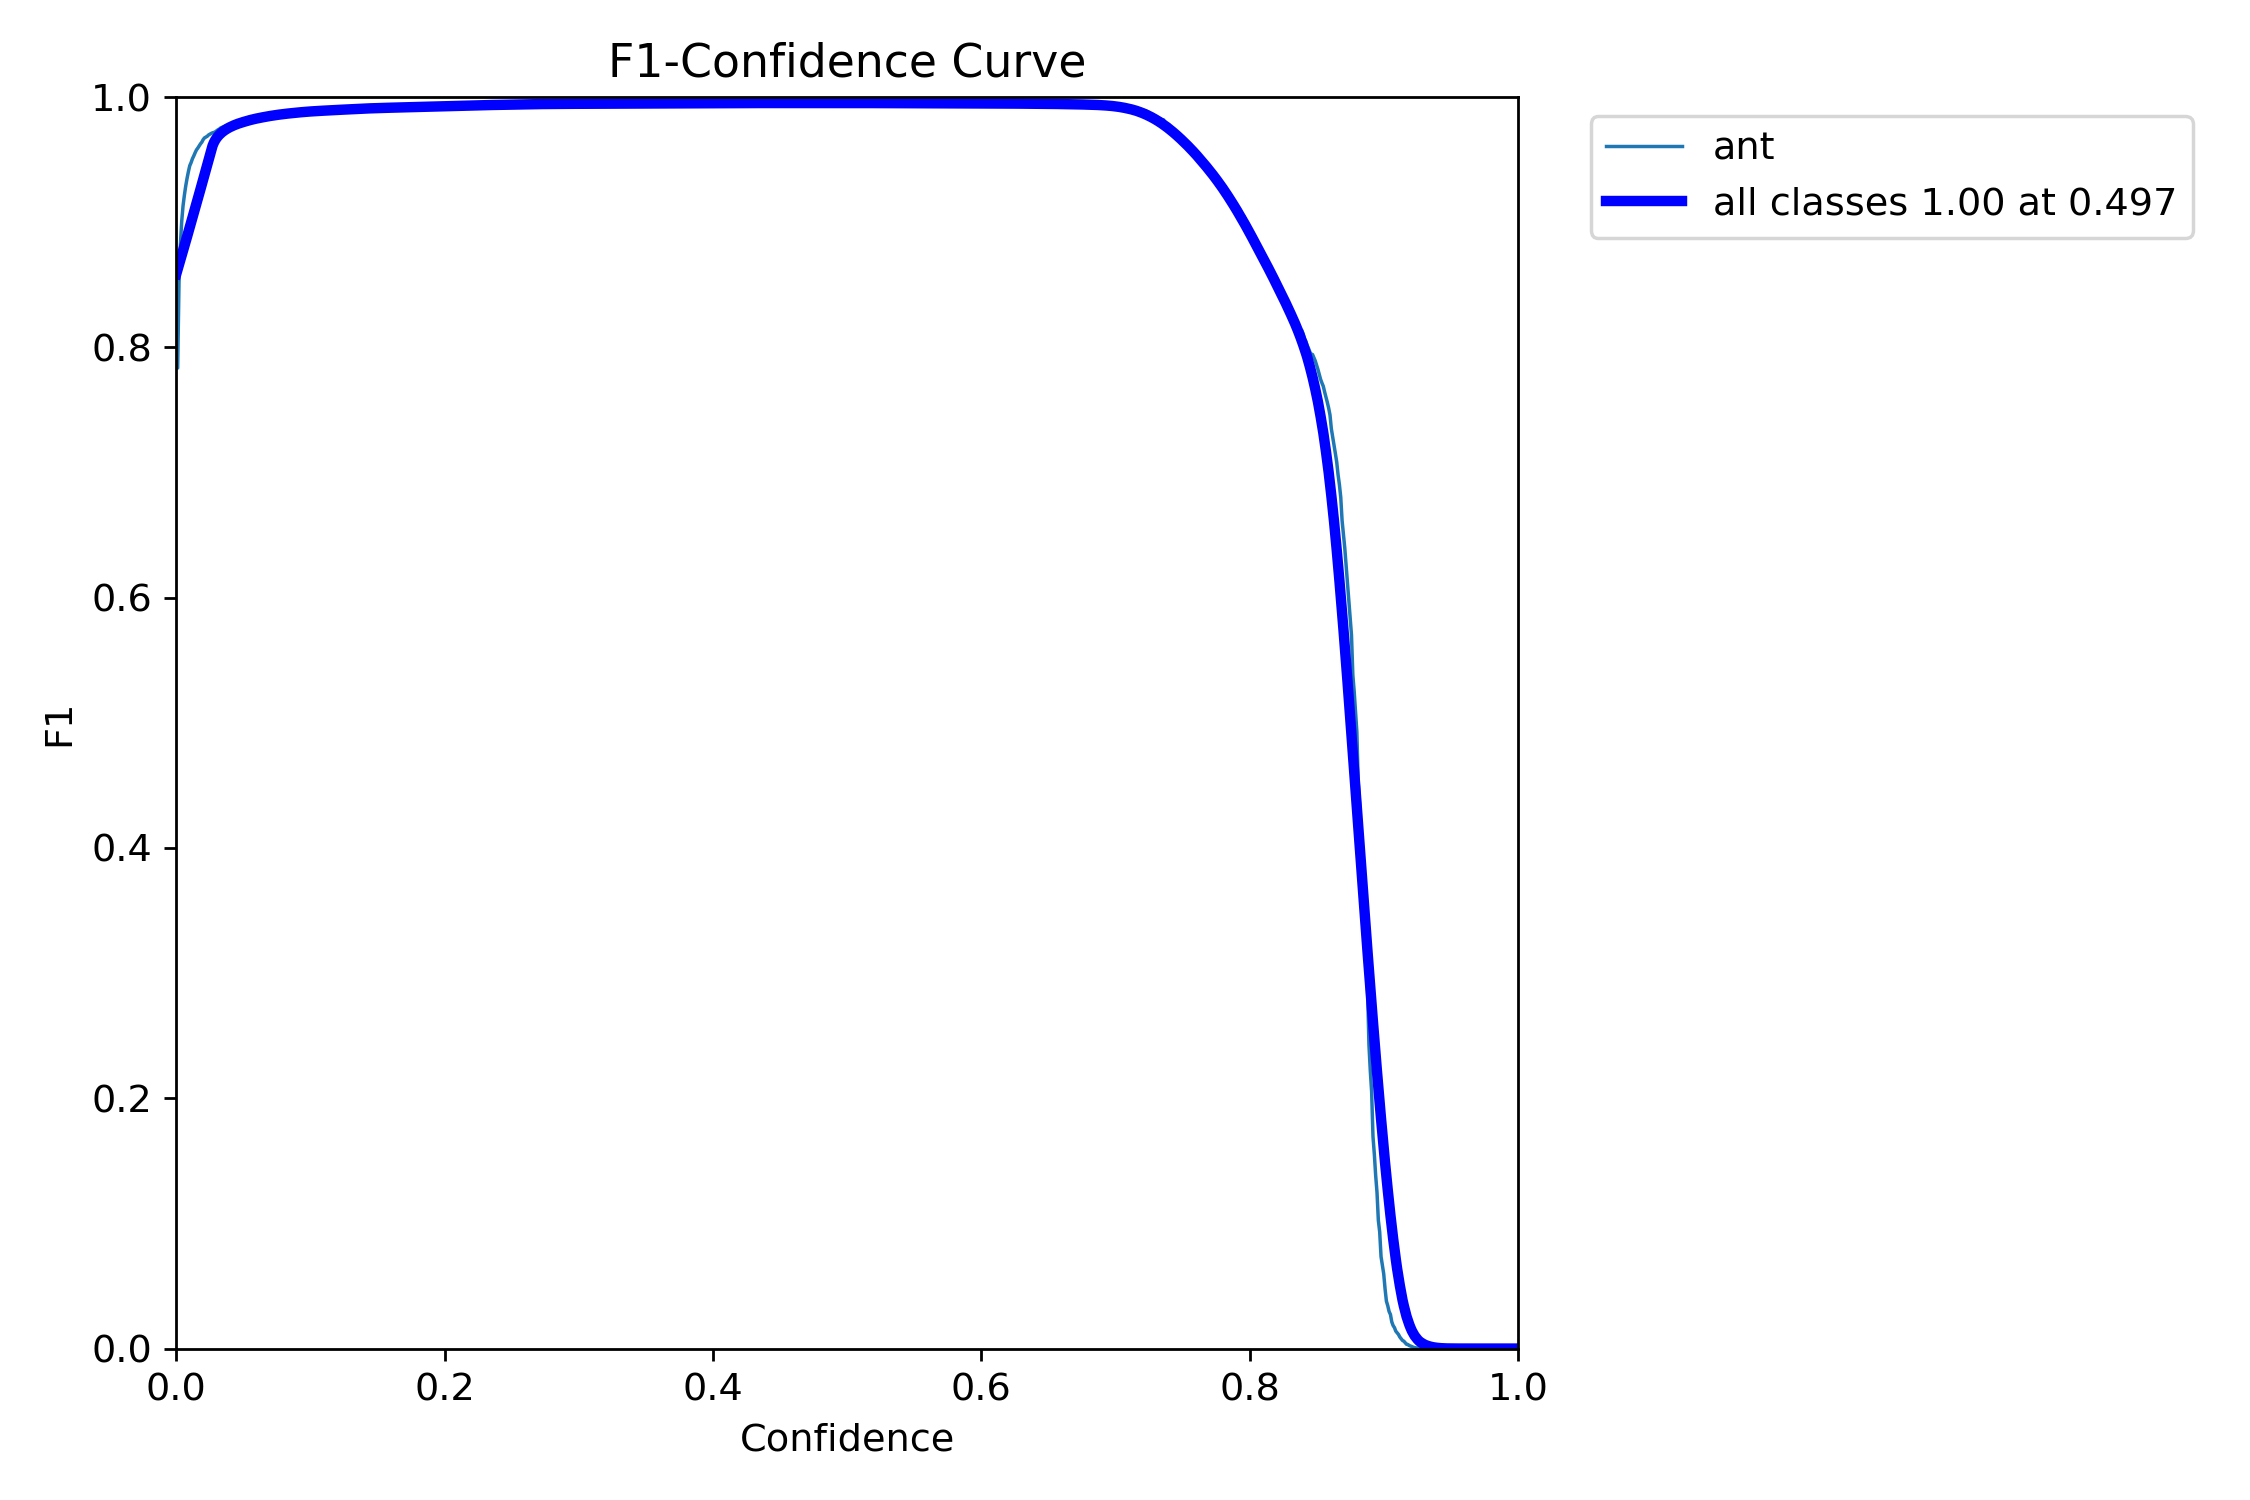
\includegraphics[width=\textwidth]{figures/06_results/F1_curveDetector.png}
        \caption[F1Score-Confidence curve of YOLOv8]{\footnotesize{F1Score-Confidence curve.}}
        \label{fig:detector_f1score}
	\end{subfigure}
	
	\caption[YOLOv8: Precision, Recall and F1Score-Confidence curve]{\footnotesize{Validation curves of the trained YOLOv8 for confidence thresholding.}}
	\label{fig:detector_precision_recall_f1}
\end{figure}
